\documentclass[tikz,fontsize=8pt,border=0pt]{standalone}
\usepackage{fourier}
\usetikzlibrary{arrows.meta}
\usetikzlibrary{calc}
\tikzset{>=latex}
\definecolor{bookblue}{RGB}{0,173,239}
\definecolor{bookpink}{RGB}{236,0,140}
\definecolor{bookgreen}{RGB}{50,200,0}
\definecolor{bookbluearea}{RGB}{204,239,252}
\tikzstyle{blueline}=[draw=bookblue,line width=0.2mm]
\tikzstyle{pinkline}=[draw=bookpink,line width=0.2mm]
\tikzstyle{greenline}=[draw=bookgreen,line width=0.2mm]
\tikzstyle{blackline}=[draw=black,line width=0.2mm]
\tikzstyle{bluearea}=[fill=bookbluearea]

\usepackage{scrextend}
\changefontsizes[8pt]{8pt}
\usetikzlibrary{decorations.pathreplacing}
\begin{document}
  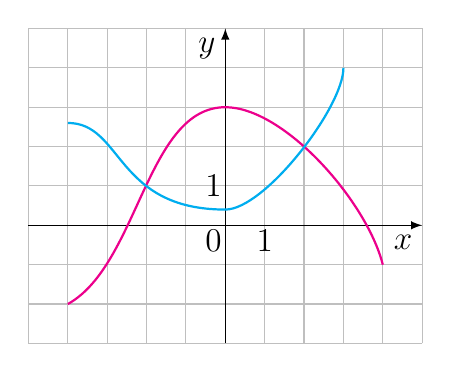
\begin{tikzpicture}
    \useasboundingbox (-2.51,-1.51) rectangle (2.51,2.51);
    \draw [step=0.5,lightgray] (-2.5,-1.5) grid (2.5,2.5);
    \node at (-0.15,-0.2) {\large 0};
    \node at (-0.15,0.5) {\large 1};
    \node at (0.5,-0.2) {\large 1};
    \draw[->] (-2.5,0) -- (2.5,0) node[below left] {\large $x$};
    \draw[->] (0,-1.5) -- (0,2.5) node[below left] {\large $y$};
    
    \draw[bookpink, thick]
    (-2,-1) .. controls (-1.1,-0.5) and (-1,1.5) .. 
    (0,1.5) .. controls (0.75,1.5) and (1.8,0.3)  .. (2,-0.5);
    
    \draw[bookblue, thick]
    (-2,1.3) .. controls (-1.3,1.3) and (-1.4,0.2) .. 
    (0,0.2) .. controls (0.5,0.2) and (1.5,1.5)  .. (1.5,2);
    
    
    %\draw [dashed, line width=0.2mm] (0.68,0) -- (0.68,0.8);
    %\draw [dashed, line width=0.2mm] (1.78,0) -- (1.78,1.38);
    
    %\draw[blackline,domain=-1.1:0.5] plot (\x+1.5,{-(\x)^2+1.5});
    %\draw[pinkline] (0.256,0.15) -- (1.356,1.91);
    %\node at (0.05,0.83) {$P(a,f(a))$};
    %\node at (1.2,2) {$t$};
    %\node at (2.1,1.7) {$Q(x, f(x))$};
    %\draw [decorate,decoration={brace,mirror},xshift=-4pt,yshift=0pt]
    %(0.85,0.78) -- (1.88,0.78) node [black,midway,yshift=-0.3cm] 
    %{\footnotesize $x-a$};
    %\draw [decorate,decoration={brace,mirror},xshift=-4pt,yshift=0pt]
    %(1.95,0.83) -- (1.95,1.38) node [black,midway,xshift=0.65cm] 
    %{\footnotesize $f(x)-f(a)$};
    %\draw[greenline] (0.7,0.83) -- (1.78,0.83);
    %\draw[greenline] (1.78,0.83) -- (1.78,1.43);
    %\draw[blueline]  (-0.3,0.3) -- (2.3,1.7);
    %\fill (0.68,0.83) circle (0.4mm);
    %\fill (1.78,1.42) circle (0.4mm);
    %\node at (0.65,-0.15) {$a$};
    %\node at (1.75,-0.15) {$x$};
  \end{tikzpicture}
\end{document}